\section{Классификация изображений датасета MNIST}

Теперь решим задачу классификации датасета MNIST. Опишем общий алгоритм \ref{classification-pipeline}, который лежит в основе решения задачи.

\medskip
\begin{algorithm}[H]
	\small
	\SetAlgoLined
	\KwData{Набор изображений рукописных цифр}
	\KwResult{Алгоритм, определяющий рукописную цифру}
	\ForEach{изображения из выборки}{
		Построить фильтрации;
		
		Найти персистентные гомологии, построить диаграмму персистентости;
		
		Получить топологические признаки из диаграммы персистентности;
	}
	
	На наборе полученных признаков обучить модель машинного обучения;
	\caption{Общий алгоритм решения задачи классификации}
	\label{classification-pipeline}
\end{algorithm}
\medskip

Как видно из алгоритма, основным этапом является получение топологических признаков. На их основе и будет обучаться модель машинного обучения. Признаки получаются из диаграммы устойчивости различными методами, поэтому для одного изображения можно получить сразу несколько признаков по одной диаграмме. С другой стороны, персистентные гомологии, а значит и диаграмму устойчивости, можно считать для различных фильтраций одного и того же изображения. Таким образом на основе одного изображения можно сразу получить большое количество признаков, строя по ней различные фильтрации и различными способами векторизуя диаграмму. В данной работе использовался подход, изображенный на рис. \ref{pipeline}

\begin{figure}[!htbp]
	\begin{center}
		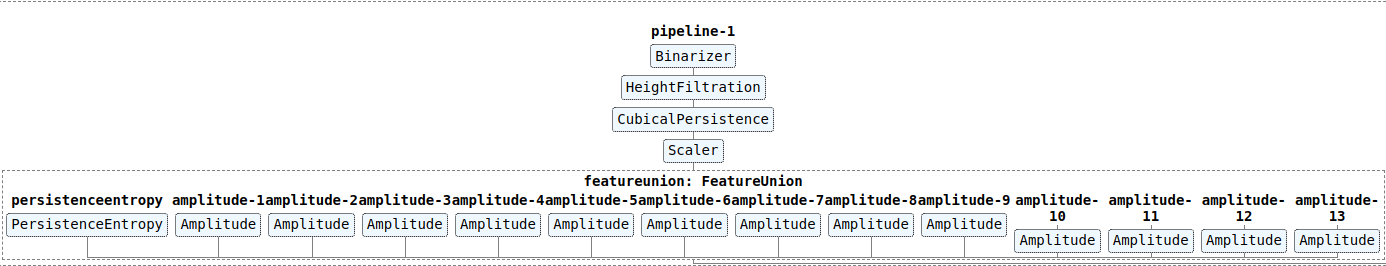
\includegraphics[width=\textwidth]{pipelineDiagram.png}\\
		\caption{Алгоритм получения признаков для Height Filtration}
		\label{pipeline}
	\end{center}
\end{figure}

Опишем подробнее алгоритм получения признаков. Первым шагом является бинаризация изображения с заранее выбранным пороговым значением(в данной работе значение порога равнялось $0.4$). Далее по бинарному изображению строятся фильтрации двумя способами: с помощью Height Filtration и Radial Filtration, причем с Height Filtration строятся 8 фильтраций, которые отличаются направлением, а с помощью Radial Filtration строятся 9 фильтраций, которые отличаются центром. Таким образом получается 17 фильтраций с одного изображения. Для каждой фильтрации получается диаграмма устойчивости, которая содержит в себе информацию о $0$ и $1$ устойчивых гомологиях, и для каждой размерности получается 14 признаков: один из признаков -- энтропия, другие -- амплитуды для различных векторных представлений диаграммы. Таким образом, для одной картинки выходит $17 \times 2 \times 14 = 476$ признаков.

Важным этапом для получения признаков является приведение диаграмм к одному и тому же масштабу. 